\documentclass{article}



% these packages let you do math
\usepackage{amsmath}
\usepackage{amssymb}

% we need these packages for fancy R tables
\usepackage{booktabs}
\usepackage{float}
\usepackage{colortbl}
\usepackage{xcolor}

% these packages play with the spacing/margins of the document. Uncomment the commands on lines 16 and 17 to see what they do.44
\usepackage{a4wide}
\usepackage{setspace}
\usepackage{geometry}
\usepackage{parskip}
\doublespacing
\geometry{margin=1.5in}

% this package helps us with including images. Setting the graphics path makes it easier to refer to things in the \includegraphics command.
\usepackage{graphicx}
\graphicspath{ {../figures/} }

% make some hyperlinks using the \href command
\usepackage{hyperref}
\hypersetup{
    colorlinks=true,
    linkcolor=black,
    urlcolor=blue
}


% set the author, title, and date of the document. \maketitle adds it to the document.
\author{Peter (Tun-Shuo) Lee }
\title{Analysis of 2002 Incarceration data from NLSY97}
\date{Sping 2022}


\begin{document}
\maketitle

\section{Introduction}

Systematic inequity between racial groups in the US has always been a widely debated topic. Differences in employment, education, income, have placed 
many families in a disadvantage that spans across generations. Amongst the racial treatment discussions, perhaps one of most contentious is of the criminal 
justice system and whether their representatives judge the cases differently based on the defendants' ethnicity. This paper will analyze the racial composition 
of the \texttt{National Longitudinal Study of Youth (NLSY)}'s data from 2002, in particular, the racial and gender distribution of the incarcerated. While this short analysis aims not to provide
a definitive conclusion to the ongoing debate, it does provide quantitative evidence on the difference (or lack there of) of incarcerations in youth across race and gender.  

\newpage

\section{Analysis}
The data set NLSY97 included 8621 individuals' gender and race information, as well as whether they were incarcerated during each month in 2002. 
By first summing the number of months, and dividing by the total number of individuals within each gender and race group, we essentially find the 
rate of incarceration of the youths for each race and gender. The data is summarized in the table below: 

\begin{table}[H]

\caption{\label{tab:tab:summarystats}Incarceration Rates in 2002 by Race and Gender}
\centering
\begin{tabular}[t]{lrrrr}
\toprule
Gender & Black & Hispanic & Mixed Race Non Hispanic & Non Black Non Hispanic\\
\midrule
\cellcolor{gray!6}{Female} & \cellcolor{gray!6}{0.0079225} & \cellcolor{gray!6}{0.0066225} & \cellcolor{gray!6}{0.0238095} & \cellcolor{gray!6}{0.0059798}\\
Male & 0.0602740 & 0.0309498 & 0.0000000 & 0.0235602\\
\bottomrule
\end{tabular}
\end{table}


An interesting trend arises in that males have a generally higher incarceration rate than females. This trend is present for all races, except for Mixed Race NonHispanic, where there are no recorded 
male incarcerations. Our findings can be better interpretted once visualized: 

\begin{figure}[H]
    \begin{center}
        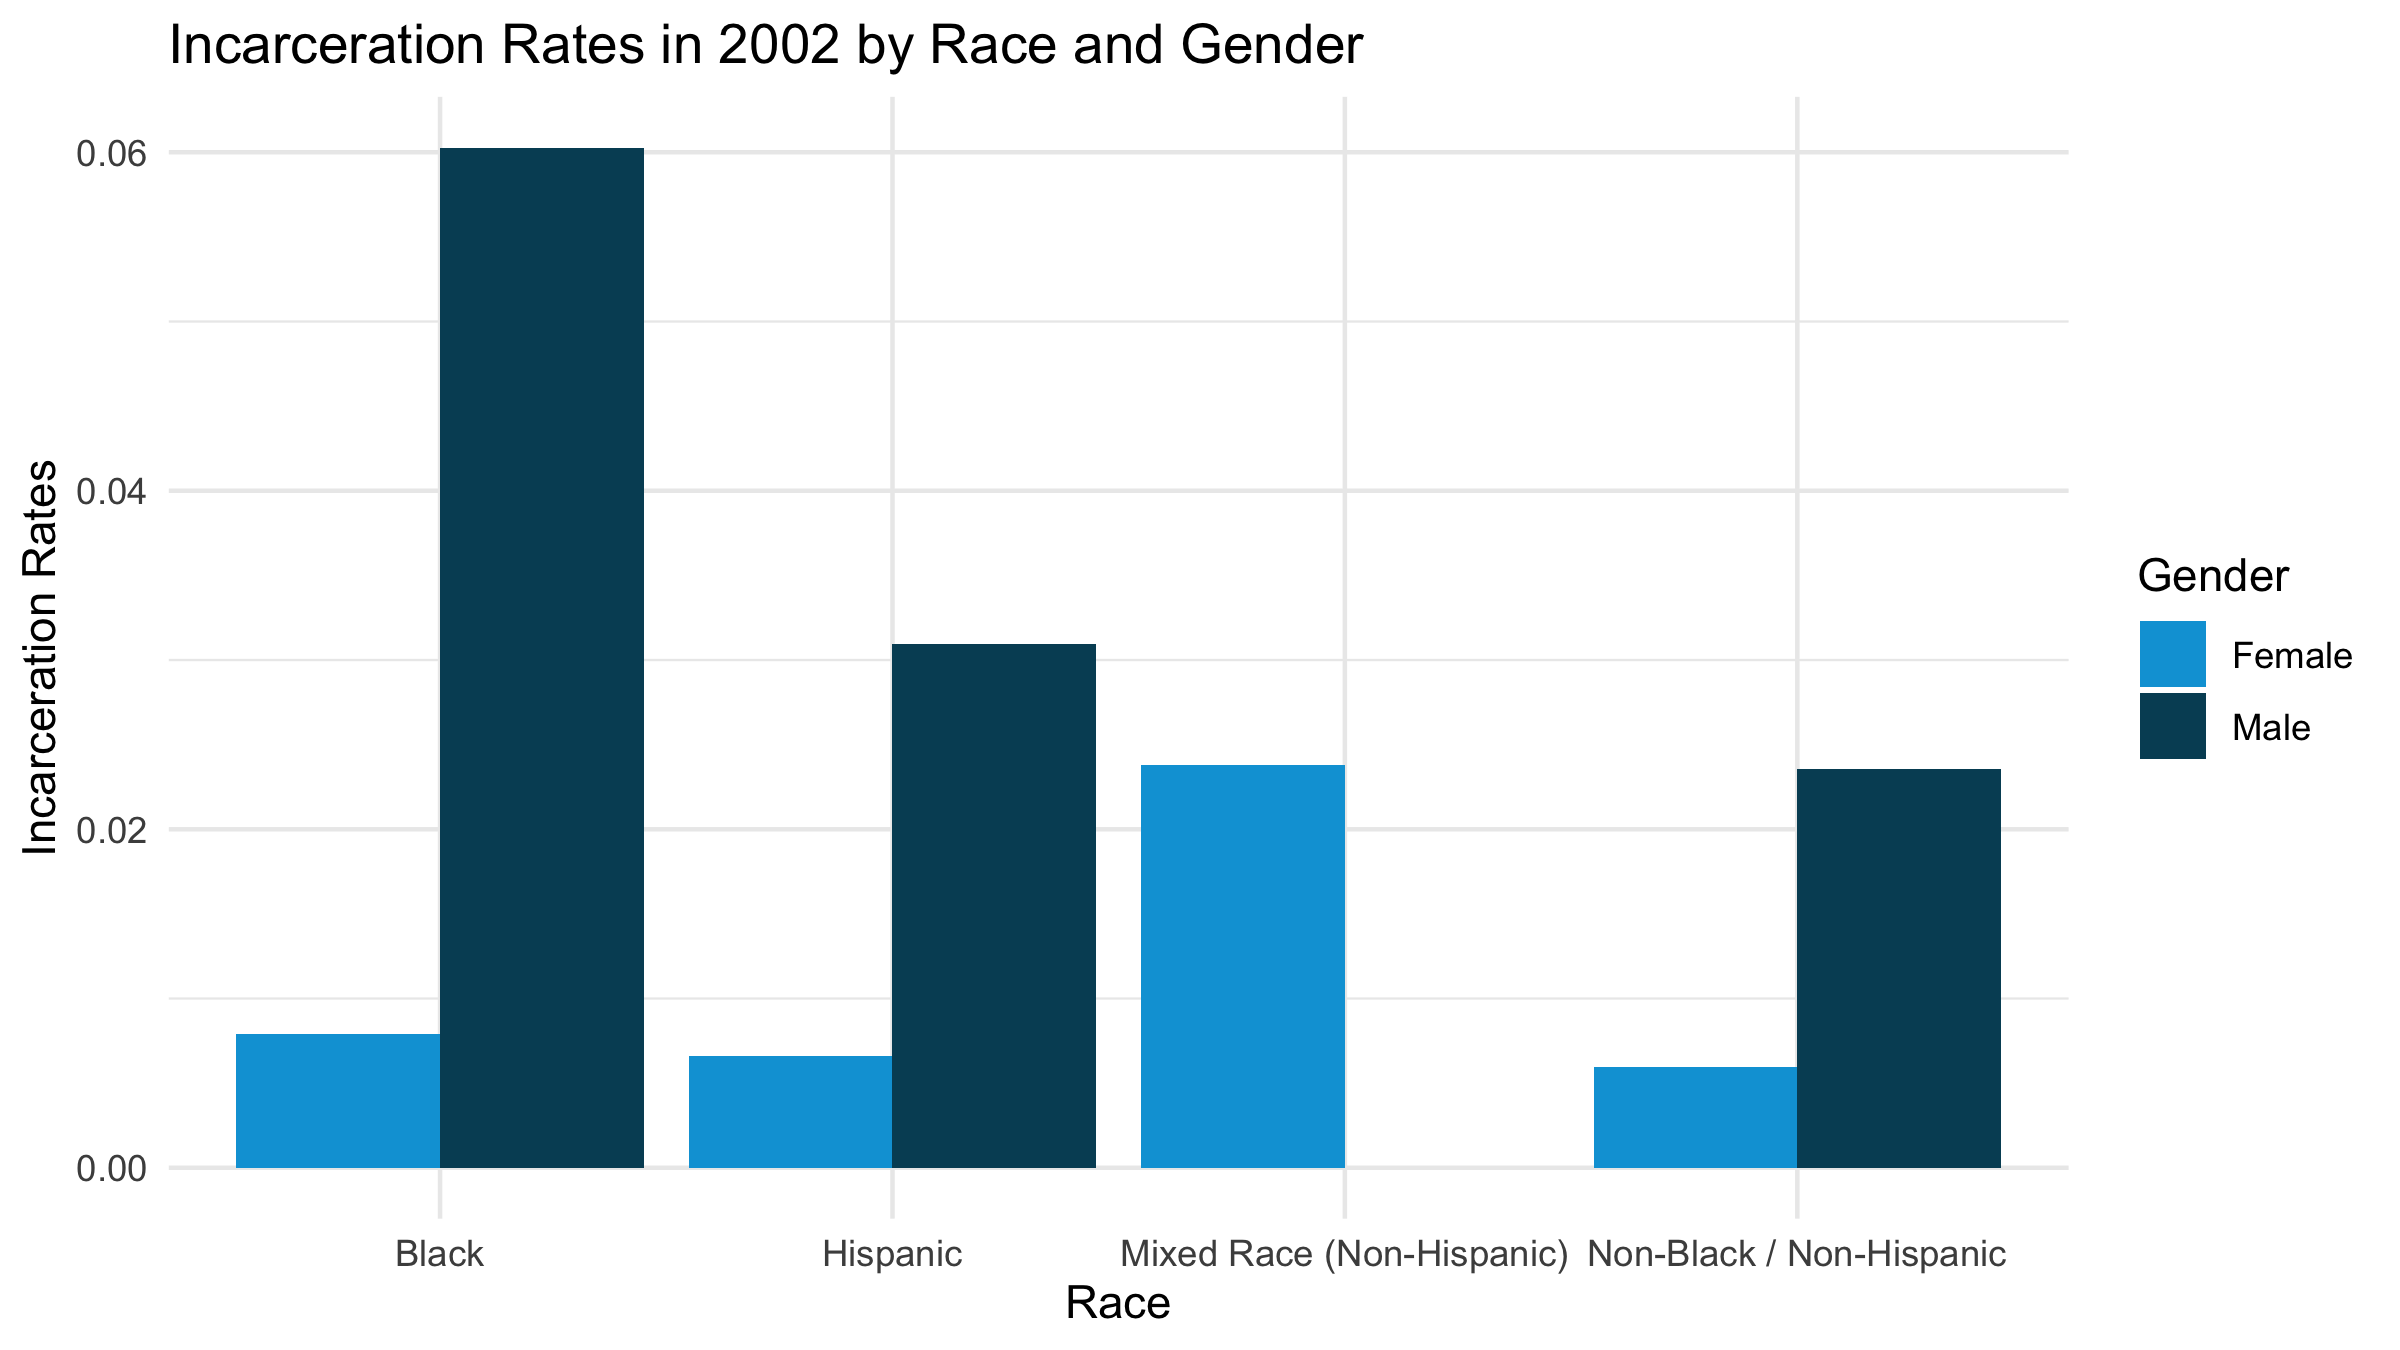
\includegraphics[width=.85\textwidth]{incarcerations_by_racegender.png}
    \end{center}
    \caption{Mean Number of Incarcerations in 2002 by Race and Gender}
    \label{fig:graph}
\end{figure}

For Black, Hispanic and Non-Black Non-Hispanic individuals, the incarceration rate for male is higher than female. The difference is the largest for Black males, then Hispanic, and the lowest being NonHispanic, NonBlack. 
With both male and female considered, Black individuals are the most likely to be incarcerated. Hispanic teens comes next, and lastly, NonBlack/ NonHispanic. Surprisingly, the incarceration rate for Mixed Raced, NonHispanic women
are higher than for women of all other races, and yet, there are no recorded incarcerations for Mixed Race, NonHispanic men. 

\section{Regression}

We regressed the incarceration rate on categorical variables representing race and gender. We omitted Black Females to avoid multicolinearity. 
$$
incarceration rate = \beta_{0} + \beta_{1}Hispanic + \beta_{2}Mixed Race (NonHispanic) + \beta_{3} NonBlack/ NonHispanic + \beta_{4} Male + \varepsilon
$$
The results are as follows: 


% Table created by stargazer v.5.2.2 by Marek Hlavac, Harvard University. E-mail: hlavac at fas.harvard.edu
% Date and time: Tue, Feb 15, 2022 - 03:52:42
\begin{table}[!htbp] \centering 
  \caption{Regression Output. Omitted category is Black Females.} 
  \label{tab:regression} 
\begin{tabular}{@{\extracolsep{5pt}}lc} 
\\[-1.8ex]\hline 
\hline \\[-1.8ex] 
 & \multicolumn{1}{c}{\textit{Dependent variable:}} \\ 
\cline{2-2} 
\\[-1.8ex] & Arrests in 2002 \\ 
\hline \\[-1.8ex] 
 Hispanic & $-$0.159$^{***}$ \\ 
  & (0.038) \\ 
  & \\ 
 Mixed Race (Non-Hispanic) & $-$0.174$^{**}$ \\ 
  & (0.083) \\ 
  & \\ 
 Non-Black / Non-Hispanic & $-$0.189$^{***}$ \\ 
  & (0.035) \\ 
  & \\ 
 Male & 0.194$^{***}$ \\ 
  & (0.022) \\ 
  & \\ 
 Constant & 0.155$^{***}$ \\ 
  & (0.026) \\ 
  & \\ 
\hline \\[-1.8ex] 
Observations & 8,621 \\ 
R$^{2}$ & 0.015 \\ 
Adjusted R$^{2}$ & 0.014 \\ 
Residual Std. Error & 1.019 (df = 8616) \\ 
F Statistic & 32.033$^{***}$ (df = 4; 8616) \\ 
\hline 
\hline \\[-1.8ex] 
\textit{Note:}  & \multicolumn{1}{r}{$^{*}$p$<$0.1; $^{**}$p$<$0.05; $^{***}$p$<$0.01} \\ 
\end{tabular} 
\end{table} 


\newpage
All coefficient values are significant at a 1\% level, except for the indicator variable for Mixed Race (NonHispanic) individuals, which is still significant at a 5\% level. The results show that there are significant differences amongst incarceration rate for individuals of different race and gender. Black women drawn from the sample are expected to have an incarceration rate of 15.5\%. On the other hand, if the random individual drawn from the sample were a man, he would be expected to have a 19.4\% higher incarceration rate than if he were female. Compared to black women, being any other race tends to have lower expected incarceration rates, with 15.9\% lower for Hispanic, 17.4\% lower for Mixed Race, and 18.9\% lower for NonBlack/NonHispanic individuals.



\section{Conclusion}

The results from the data shows that there exists differences in incarceration rates based on gender and race. In particular, men are expected to have higher incarceration rates, and black individuals have the highest incarceration rates of all the other races; however, there only exists correlation. The paper's evidence cannot support, nor deny the existence of race based discrimination in the American Judicial System. 

The analysis solely provides qualitative evidence, and illustrates the simple fact that there exists a difference. Since variables like income, family size, education levels, drug use, and other affiliated variables are omitted, the estimated coefficients may suffer from omitted variable bias, making attributing the difference in incarceration rates to gender and race. 

More insights may be revealed when socioeconomic and economic factors are considered. As low education rates, and access to drugs often drive an individual to pursue illegal activities, I suspect their effects would reduce the differences amongst individuals of different race. This IS after all a debate rooted in the socioeconomic and economic differences between races, and those same factors would still contribute to the higher incarceration rate for certain races even when the court were truly impartial. The evidence of this paper is not able to differentiate between higher incarceration rates purely due to biased a judicial system, and due to the actual just rulings for crimes that are disporportionally committed more by members of certain races. Further studies and expansions on the current methodology are required to answer the question. These future studies may also identify opporutnities and alternative improvements to the incarceration of teens other than incarceration such as improved access to education, food security, and healthcare.

\end{document}